\section*{ouverture}
\paragraph{}
Le large succès de Wikipedia et le progrès des techniques d’extraction des données ont abouti à la naissance de la construction automatique  de larges base de connaissances comme DBpedia, YAGO, etc...
\subparagraph{}
Beaucoup de connaissances sont construites en se basant sur l’extraction automatique des faits relationnels dans un texte.
Malheureusement, les bases de connaissances convergent sur les faits statiques et ne donnent pas une grande importance à la dimension temporelle.
Malgré le fait que la majorité des faits évoluent avec le temps, ou n'est valide que dans une période temporelle précise.
Ainsi, nous remarquons que le temps a une dimension significatif dans des bases de connaissances comme DBpedia.
\subparagraph{}
Dans cette étude on veut extraire des faits temporels et des évènements depuis des information semi-structurées de Wikipedia et Wikidata ; et textuelles de Wikipedia.
\paragraph{}
La dimension temporelle est particulièrement importante dans les relations binaires comme isPresidentOf, isCEOof, isMarriedTo, on peut être mariée à plusieurs épouses mais dans des différents intervalles de temps mais “On ne prend pas compte des exceptions de mariage polygames ”.
\subparagraph{}
Une base de connaissance contenant plusieurs présidents des États-Unis ne peut être consistante que lorsqu’on ajoute une dimension temporelle à ces faits. De plus l’annotation temporelle aide à faire la distinction entre les faits courants et et les faits dépassés.
Par exemple le fait “Kennedy est le président des États-Unis” est correct, mais n'est plus valide.
Lorsqu’on attache une annotation temporelle à un fait comme celui là, il devient universellement valide.
\subsection*{Extraction}
\paragraph{}
Les faits temporels extraites de Wikipedia consiste en deux phases principales : extractions des données semi-structurées(tableaux, infoboxes) et l’extraction depuis le texte wikipédia.
\subparagraph{}
Les infoboxes : Contiennent généralement les informations les plus importantes des entités décrites dans l’article. Par exemple dans l’infobox de “Kennedy” l’ancien président des États-Unis sur wikipédia on trouve la date d’élection, le prédécesseur du président, la durée du mandat, etc…
\newline
Chaque infoBox a un type particulier comme: évènement historique, élection, compétition ect…
\subparagraph{}
Modèle quaternaire : un modèle qui capte la base du fait avec un indice temporel.
\newline
<politician> served as <politician office> from <date> to <date>
\newline
f1: Kennedy holdsPoliticalPosition PresidentOfUSA 
\newline
f2:f1 startedOnDate 
\newline
f3:f1 endedOnDate
\newline
HappenedDate est utilisée pour dire que le fait est valide que dans ce point du temps.
\begin{figure}[H]
        \centering
                \centering
                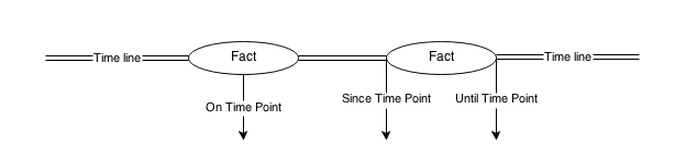
\includegraphics[width=10cm]{timeline.png}
               \caption{Event Time Line}

\end{figure}
\subparagraph{}
Certes, on peut créer des “patterns” parton ou motifs à travers les faits temporels dans la base de connaissances mais on cherche ici à extraire les informations des textes et des données semi-structurée afin de leur trouver une autre structure plus adéquate (tel un triplet annoter ou bien un quadrupet).